
\section{\NP-completeness and connected pages}

\begin{frame}{\probBook is \NP-complete}

\begin{theorem}
\probBook with matchings as pages is \NP-complete.
\end{theorem}

Reduce from \NP-complete problem \probBetween [Opatrny, 1979].
\newProb{\probBetween}{Finite set $M := \range{n}$ and ordered triples $C \subseteq M^3$.}
{Is there a total ordering $<$ of $M$ such that $a < b < c$ or $a > b > c$ for all $(a, b, c) \in C$?}
\end{frame}

\begin{frame}{Reduction from \probBetween}

\newProb{\probBetween}{Finite set $M := \range{n}$ and ordered triples $C \subseteq M^3$.}
{Is there a total ordering $<$ of $M$ such that $a < b < c$ or $a > b > c$ for all $(a, b, c) \in C$?}

Map triple~$(a, b, c) \in C$ to two new pages ($r$ fixed new vertex):	
\begin{figure}
\centering

\begin{tikzpicture}
% a < b < c
\node (r) {r};
\node [right of=r] (a) {a};
\node [right of=a] (b) {b};
\node [right of=b] (c) {c};

\draw[edge1] (r) edge [bend right] (a);
\draw[edge1] (b) edge [bend right] (c);
\draw (a) edge [bend left]  (b);
\draw (r) edge [bend left]  (c);  
\end{tikzpicture}

\end{figure}

\begin{overprint}
\onslide<1>
For example: $(a, b, c)$, $(b, c, d)$
\begin{figure}\centering
\begin{tikzpicture}
% a < b < c
\node (r) {r};
\node [right of=r] (a) {a};
\node [right of=a] (b) {b};
\node [right of=b] (c) {c};
\node [right of=c] (d) {d};

\drawedges[bend left]{r/a,b/c};
\drawedges[bend left,edge2]{r/b,c/d};
\drawedges[bend right,edge1]{a/b,r/c};
\drawedges[bend right,edge3]{b/c,r/d};
\end{tikzpicture}
\end{figure}

\onslide<2>
\probBetween $\Rightarrow$ \probBook:\\
Take~$r$ as first vertex\\
$\rightsquigarrow$ Orders $r < a < b < c$ or $r < c < b < a$ are valid

\onslide<3>
\probBook $\Rightarrow$ \probBetween:\\
Rotate $r$ to front\\
$\rightsquigarrow$ $r < a < b < c$ or $r < c < b < a$ are the only valid orders

\end{overprint}
\end{frame}



\begin{frame}<1>[label=connected,fragile]{Connected pages}

\begin{theorem}
\probBook with connected pages can be solved in $\OO(kn)$~time.
\end{theorem}

\begin{overprint}
\onslide<1>
Idea:\\Compute valid orders $\pi_i \subseteq \Sym(n)$ for single pages and\\intersect them.

\begin{figure}\centering
\resizebox{0.3\textwidth}{!}{
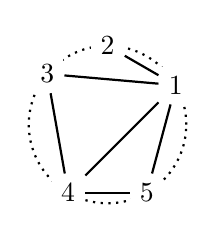
\begin{tikzpicture}
    \tikzstyle{every node}+=[fill=white]
	\draw[dotted] (0, 0) circle (1);
	\node (1) at (30:1) {1};
    \node (2) at (90:1) {2};
	\node (3) at (140:1) {3};
	\node (4) at (240:1) {4};
	\node (5) at (300:1) {5};
	\drawedges{1/2,3/4,1/3,1/4,1/5,4/5};
	\draw (1) -- (2);
	\draw (3) -- (4);
	\draw (1) -- (3);
	\draw (1) -- (4);
	\draw (1) -- (5);
	\draw (4) -- (5);
\end{tikzpicture}
}
\end{figure}

\onslide<2>

\begin{itemize}
\item Construct \PQ-trees $T_i$ on~$V$ representing valid orders of individual pages
$(V,E_i)$\hfill$\OO(n)$
\begin{figure}
\centering
\resizebox{0.6\textwidth}{!}{
\begin{tikzpicture}
\path[use as bounding box] (-2,2) rectangle (8,-2.5);

\tikzstyle{every node}+=[minimum size=0.5cm,thick]
\tikzstyle{every path}+=[thick]

\node[] (a) {$a$};
\node[right of=a] (b) {$b$};
\node[below of=b] (c) {$c$};
\node[left of=c] (d) {$d$};
\node[left of=a, above of=a] (r) {$r$};

\draw (a) edge (b) 
      (b) edge (c) 
      (c) edge (d) 
      (d) edge (a);
\draw[dashed] (r) edge (a)
              (r) edge (b)
              (r) edge (d)
              (r) edge[out=270, in=270, min distance=6em] (c);

% PQ-tree
\begin{scope}[xshift=5cm]
\node[draw,rectangle,minimum size=.2cm] {}
   child {node {$a$}}
   child {node {$b$}}
   child {node {$c$}}
   child {node {$d$}};
\end{scope}
\end{tikzpicture}}
\end{figure}

[Booth and Lueker et. al. 1976, Shih and Hsu 1993,\\Boyer and Myrvold 1999]
\end{itemize}

\onslide<3>
\begin{itemize}
\item Construct \PQ-trees $T_i$ on~$V$ representing valid orders of individual pages
$(V,E_i)$\hfill$\OO(n)$
\item Intersect the $T_i$ [Booth, 1975]\hfill$\OO(n)$
\item[$\rightarrow$] Resulting \PQ-tree~$T$ represents valid book orders
\end{itemize}
\end{overprint}

\end{frame} 

\begin{frame}{Interludium: \PQ-trees}

\begin{overprint}
\onslide<1>
$\hspace{4em}T = 
\begin{aligned}
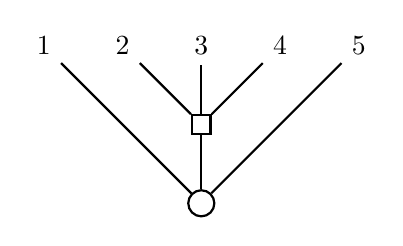
\begin{tikzpicture}

\tikzstyle{every path}+=[thick]

\node (1) {1};
\node[right of=1] (2) {2};
\node[right of=2] (3) {3};
\node[right of=3] (4) {4};
\node[right of=4] (5) {5};

\node[rectangle, draw, below of=3] (t2) {};
\node[circle, draw, below of=t2] (t1) {};

\draw (t1) edge (1);
\draw (t1) edge (5);
\draw (t2) edge (2);
\draw (t2) edge (3);
\draw (t2) edge (4);
\draw (t1) edge (t2);
\end{tikzpicture}
\end{aligned}$

\onslide<2>
$\hspace{4em}T = 
\begin{aligned}
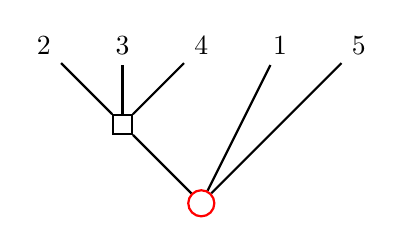
\begin{tikzpicture}

\tikzstyle{every path}+=[thick]

\node (2) {2};
\node[right of=2] (3) {3};
\node[right of=3] (4) {4};
\node[right of=4] (1) {1};
\node[right of=1] (5) {5};

\node[rectangle, draw, below of=3] (t2) {};
\node[circle, draw, below of=t2,right of=t2,red] (t1) {};

\draw (t1) edge (1);
\draw (t1) edge (5);
\draw (t2) edge (2);
\draw (t2) edge (3);
\draw (t2) edge (4);
\draw (t1) edge (t2);
\end{tikzpicture}
\end{aligned}$

\onslide<3>
$\hspace{4em}T = 
\begin{aligned}
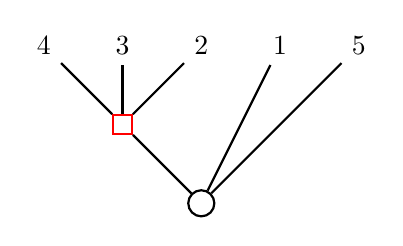
\begin{tikzpicture}

\tikzstyle{every path}+=[thick]

\node (4) {4};
\node[right of=4] (3) {3};
\node[right of=3] (2) {2};
\node[right of=2] (1) {1};
\node[right of=1] (5) {5};

\node[rectangle, draw, below of=3,red] (t2) {};
\node[circle, draw, below of=t2,right of=t2] (t1) {};

\draw (t1) edge (1);
\draw (t1) edge (5);
\draw (t2) edge (2);
\draw (t2) edge (3);
\draw (t2) edge (4);
\draw (t1) edge (t2);
\end{tikzpicture}
\end{aligned}$

\onslide<4>
$\hspace{4em}T = 
\begin{aligned}
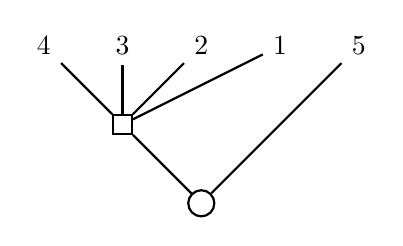
\begin{tikzpicture}

\tikzstyle{every path}+=[thick]

\node (4) {4};
\node[right of=4] (3) {3};
\node[right of=3] (2) {2};
\node[right of=2] (1) {1};
\node[right of=1] (5) {5};

\node[rectangle, draw, below of=3] (t2) {};
\node[circle, draw, below of=t2,right of=t2] (t1) {};

\draw (t2) edge (1);
\draw (t1) edge (5);
\draw (t2) edge (2);
\draw (t2) edge (3);
\draw (t2) edge (4);
\draw (t1) edge (t2);
\end{tikzpicture}
\end{aligned}$
\end{overprint}


\begin{overprint}
\onslide<1-3>
\begin{align*}
\pi(T) & = \{\only<1>{\alert{12345}}\only<2->{12345}, 14325, 52341, 54321, 15234, 15432, \\
         & \hspace{1.8em} 51234, 51432, \only<2>{\alert{23415}}\only<1,3->{23415}, \only<3>{\alert{43215}}\only<1-2>{43215}, 23451, 43251\}
\end{align*}

\onslide<4>
\begin{align*}
\pi(T) & = \{\alert{12345}, 14325, 52341, \alert{54321}, 15234, 15432, \\
         & \hspace{1.8em} \alert{51234}, 51432, 23415, \alert{43215}, 23451, 43251\}
\end{align*}
Permutations with the leaves in $\{1, 2\}$ adjacent
\end{overprint}
\end{frame}

\againframe{connected}

\resultFrame{3}